\section{Versuch}

Es soll die molare Wärmekapazität in Abhängigkeit der Temperatur gemessen werden.
Dazu wird eine Kupferprobe zunächst auf \SI{80}{\kelvin} abgekühlt.
Anschließend wird kontrolliert Energie zugeführt und sowohl die Energiemenge als auch der Temperaturanstieg gemessen.

\begin{figure}
	\centering
	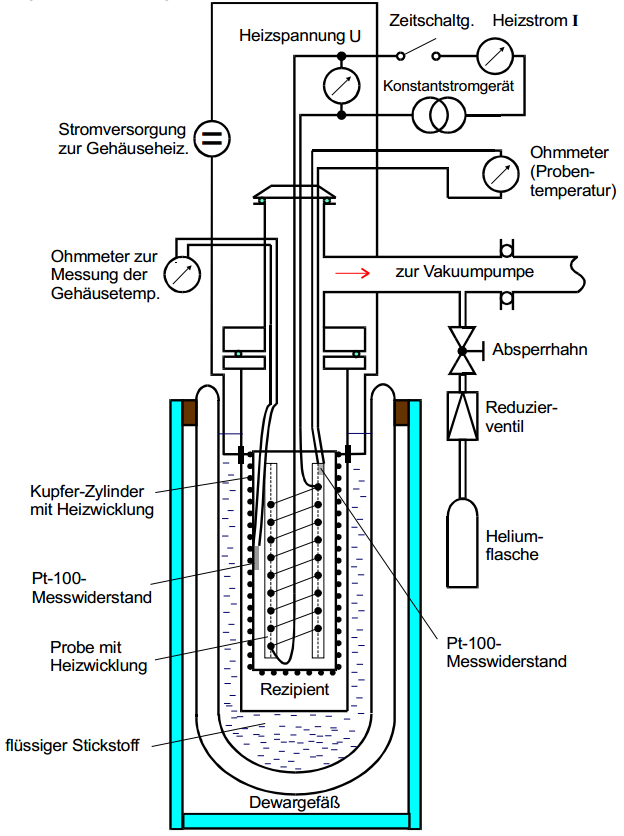
\includegraphics[width=0.8\textwidth]{img/aufbau.png}
	\caption{Versuchsaufbau \cite{v47}}
	\label{fig:aufbau}
\end{figure}

Der Versuchsaufbau ist in Abbildung \ref{fig:aufbau} dargestellt. Die Probe befindet sich in einem Rezipienten, der wiederum in einem Dewargefäß aufgehängt ist.
Zum Abkühlen der Probe wird flüssiger Stickstoff in das Dewargefäß gefüllt.
Während des Abkühlvorgangs ist der Rezipient mit Helium gefüllt, um den Wärmeübertrag zu erleichtern.

Während der Messung wird die Probe mit einer Heizwicklung erhitzt.
Die angelegte Spannung und der Strom werden dabei aufgenommen, um die Heizleistung zu berechnen.
Zwei Pt-100-Messwiderstände sind an der Probe und am Rezipienten angebracht, mit dem die Temperaturen gemessen werden.

Es soll vermieden werden, dass der Probe, abgesehen von der kontrollierten Erwärmung, Wärme zugeführt wird.
Dazu wird der Rezipient mit einer Vakuumpumpe evakuiert.
Weiterhin wird mit einer zweiten Heizwicklung der Rezipient erhitzt, sodass der Temperaturunterschied zwischen Rezipient und Probe möglichst gering ist.

Die Probe wird in Intervallen von $\SI{7}{\degree} - \SI{11}{\degree}$ erhitzt.
Zwischen den Intervallen wird ggf. der Heizstrom angepasst.